% GNUPLOT: LaTeX picture with Postscript
\begingroup
  \makeatletter
  \providecommand\color[2][]{%
    \GenericError{(gnuplot) \space\space\space\@spaces}{%
      Package color not loaded in conjunction with
      terminal option `colourtext'%
    }{See the gnuplot documentation for explanation.%
    }{Either use 'blacktext' in gnuplot or load the package
      color.sty in LaTeX.}%
    \renewcommand\color[2][]{}%
  }%
  \providecommand\includegraphics[2][]{%
    \GenericError{(gnuplot) \space\space\space\@spaces}{%
      Package graphicx or graphics not loaded%
    }{See the gnuplot documentation for explanation.%
    }{The gnuplot epslatex terminal needs graphicx.sty or graphics.sty.}%
    \renewcommand\includegraphics[2][]{}%
  }%
  \providecommand\rotatebox[2]{#2}%
  \@ifundefined{ifGPcolor}{%
    \newif\ifGPcolor
    \GPcolorfalse
  }{}%
  \@ifundefined{ifGPblacktext}{%
    \newif\ifGPblacktext
    \GPblacktexttrue
  }{}%
  % define a \g@addto@macro without @ in the name:
  \let\gplgaddtomacro\g@addto@macro
  % define empty templates for all commands taking text:
  \gdef\gplbacktext{}%
  \gdef\gplfronttext{}%
  \makeatother
  \ifGPblacktext
    % no textcolor at all
    \def\colorrgb#1{}%
    \def\colorgray#1{}%
  \else
    % gray or color?
    \ifGPcolor
      \def\colorrgb#1{\color[rgb]{#1}}%
      \def\colorgray#1{\color[gray]{#1}}%
      \expandafter\def\csname LTw\endcsname{\color{white}}%
      \expandafter\def\csname LTb\endcsname{\color{black}}%
      \expandafter\def\csname LTa\endcsname{\color{black}}%
      \expandafter\def\csname LT0\endcsname{\color[rgb]{1,0,0}}%
      \expandafter\def\csname LT1\endcsname{\color[rgb]{0,1,0}}%
      \expandafter\def\csname LT2\endcsname{\color[rgb]{0,0,1}}%
      \expandafter\def\csname LT3\endcsname{\color[rgb]{1,0,1}}%
      \expandafter\def\csname LT4\endcsname{\color[rgb]{0,1,1}}%
      \expandafter\def\csname LT5\endcsname{\color[rgb]{1,1,0}}%
      \expandafter\def\csname LT6\endcsname{\color[rgb]{0,0,0}}%
      \expandafter\def\csname LT7\endcsname{\color[rgb]{1,0.3,0}}%
      \expandafter\def\csname LT8\endcsname{\color[rgb]{0.5,0.5,0.5}}%
    \else
      % gray
      \def\colorrgb#1{\color{black}}%
      \def\colorgray#1{\color[gray]{#1}}%
      \expandafter\def\csname LTw\endcsname{\color{white}}%
      \expandafter\def\csname LTb\endcsname{\color{black}}%
      \expandafter\def\csname LTa\endcsname{\color{black}}%
      \expandafter\def\csname LT0\endcsname{\color{black}}%
      \expandafter\def\csname LT1\endcsname{\color{black}}%
      \expandafter\def\csname LT2\endcsname{\color{black}}%
      \expandafter\def\csname LT3\endcsname{\color{black}}%
      \expandafter\def\csname LT4\endcsname{\color{black}}%
      \expandafter\def\csname LT5\endcsname{\color{black}}%
      \expandafter\def\csname LT6\endcsname{\color{black}}%
      \expandafter\def\csname LT7\endcsname{\color{black}}%
      \expandafter\def\csname LT8\endcsname{\color{black}}%
    \fi
  \fi
    \setlength{\unitlength}{0.0500bp}%
    \ifx\gptboxheight\undefined%
      \newlength{\gptboxheight}%
      \newlength{\gptboxwidth}%
      \newsavebox{\gptboxtext}%
    \fi%
    \setlength{\fboxrule}{0.5pt}%
    \setlength{\fboxsep}{1pt}%
\begin{picture}(5668.00,3968.00)%
    \gplgaddtomacro\gplbacktext{%
      \csname LTb\endcsname%%
      \put(434,3171){\makebox(0,0)[r]{\strut{}$0$}}%
      \csname LTb\endcsname%%
      \put(434,3511){\makebox(0,0)[r]{\strut{}$0.9$}}%
      \csname LTb\endcsname%%
      \put(434,3851){\makebox(0,0)[r]{\strut{}$1.8$}}%
      \csname LTb\endcsname%%
      \put(566,2875){\makebox(0,0){\strut{}}}%
      \csname LTb\endcsname%%
      \put(1101,2875){\makebox(0,0){\strut{}}}%
      \csname LTb\endcsname%%
      \put(1636,2875){\makebox(0,0){\strut{}}}%
      \csname LTb\endcsname%%
      \put(2172,2875){\makebox(0,0){\strut{}}}%
      \csname LTb\endcsname%%
      \put(2707,2875){\makebox(0,0){\strut{}}}%
      \csname LTb\endcsname%%
      \put(3242,2875){\makebox(0,0){\strut{}}}%
      \csname LTb\endcsname%%
      \put(3777,2875){\makebox(0,0){\strut{}}}%
      \csname LTb\endcsname%%
      \put(4313,2875){\makebox(0,0){\strut{}}}%
      \csname LTb\endcsname%%
      \put(4848,2875){\makebox(0,0){\strut{}}}%
      \csname LTb\endcsname%%
      \put(5383,2875){\makebox(0,0){\strut{}}}%
    }%
    \gplgaddtomacro\gplfronttext{%
      \csname LTb\endcsname%%
      \put(-171,3511){\rotatebox{-270}{\makebox(0,0){\strut{}$V_{out,and}$}}}%
      \put(2974,2809){\makebox(0,0){\strut{}}}%
    }%
    \gplgaddtomacro\gplbacktext{%
      \csname LTb\endcsname%%
      \put(434,2337){\makebox(0,0)[r]{\strut{}$0$}}%
      \csname LTb\endcsname%%
      \put(434,2678){\makebox(0,0)[r]{\strut{}$0.9$}}%
      \csname LTb\endcsname%%
      \put(434,3018){\makebox(0,0)[r]{\strut{}$1.8$}}%
      \csname LTb\endcsname%%
      \put(566,2041){\makebox(0,0){\strut{}}}%
      \csname LTb\endcsname%%
      \put(1101,2041){\makebox(0,0){\strut{}}}%
      \csname LTb\endcsname%%
      \put(1636,2041){\makebox(0,0){\strut{}}}%
      \csname LTb\endcsname%%
      \put(2172,2041){\makebox(0,0){\strut{}}}%
      \csname LTb\endcsname%%
      \put(2707,2041){\makebox(0,0){\strut{}}}%
      \csname LTb\endcsname%%
      \put(3242,2041){\makebox(0,0){\strut{}}}%
      \csname LTb\endcsname%%
      \put(3777,2041){\makebox(0,0){\strut{}}}%
      \csname LTb\endcsname%%
      \put(4313,2041){\makebox(0,0){\strut{}}}%
      \csname LTb\endcsname%%
      \put(4848,2041){\makebox(0,0){\strut{}}}%
      \csname LTb\endcsname%%
      \put(5383,2041){\makebox(0,0){\strut{}}}%
    }%
    \gplgaddtomacro\gplfronttext{%
      \csname LTb\endcsname%%
      \put(-171,2677){\rotatebox{-270}{\makebox(0,0){\strut{}$V_{out,or}$}}}%
      \put(2974,1975){\makebox(0,0){\strut{}}}%
    }%
    \gplgaddtomacro\gplbacktext{%
      \csname LTb\endcsname%%
      \put(434,1504){\makebox(0,0)[r]{\strut{}$0$}}%
      \csname LTb\endcsname%%
      \put(434,1845){\makebox(0,0)[r]{\strut{}$0.9$}}%
      \csname LTb\endcsname%%
      \put(434,2185){\makebox(0,0)[r]{\strut{}$1.8$}}%
      \csname LTb\endcsname%%
      \put(566,1208){\makebox(0,0){\strut{}}}%
      \csname LTb\endcsname%%
      \put(1101,1208){\makebox(0,0){\strut{}}}%
      \csname LTb\endcsname%%
      \put(1636,1208){\makebox(0,0){\strut{}}}%
      \csname LTb\endcsname%%
      \put(2172,1208){\makebox(0,0){\strut{}}}%
      \csname LTb\endcsname%%
      \put(2707,1208){\makebox(0,0){\strut{}}}%
      \csname LTb\endcsname%%
      \put(3242,1208){\makebox(0,0){\strut{}}}%
      \csname LTb\endcsname%%
      \put(3777,1208){\makebox(0,0){\strut{}}}%
      \csname LTb\endcsname%%
      \put(4313,1208){\makebox(0,0){\strut{}}}%
      \csname LTb\endcsname%%
      \put(4848,1208){\makebox(0,0){\strut{}}}%
      \csname LTb\endcsname%%
      \put(5383,1208){\makebox(0,0){\strut{}}}%
    }%
    \gplgaddtomacro\gplfronttext{%
      \csname LTb\endcsname%%
      \put(-171,1844){\rotatebox{-270}{\makebox(0,0){\strut{}$V_{in,1}$}}}%
      \put(2974,1142){\makebox(0,0){\strut{}}}%
    }%
    \gplgaddtomacro\gplbacktext{%
      \csname LTb\endcsname%%
      \put(434,671){\makebox(0,0)[r]{\strut{}$0$}}%
      \csname LTb\endcsname%%
      \put(434,1012){\makebox(0,0)[r]{\strut{}$0.9$}}%
      \csname LTb\endcsname%%
      \put(434,1352){\makebox(0,0)[r]{\strut{}$1.8$}}%
      \csname LTb\endcsname%%
      \put(566,375){\makebox(0,0){\strut{}0}}%
      \csname LTb\endcsname%%
      \put(1101,375){\makebox(0,0){\strut{}10}}%
      \csname LTb\endcsname%%
      \put(1636,375){\makebox(0,0){\strut{}20}}%
      \csname LTb\endcsname%%
      \put(2172,375){\makebox(0,0){\strut{}30}}%
      \csname LTb\endcsname%%
      \put(2707,375){\makebox(0,0){\strut{}40}}%
      \csname LTb\endcsname%%
      \put(3242,375){\makebox(0,0){\strut{}50}}%
      \csname LTb\endcsname%%
      \put(3777,375){\makebox(0,0){\strut{}60}}%
      \csname LTb\endcsname%%
      \put(4313,375){\makebox(0,0){\strut{}70}}%
      \csname LTb\endcsname%%
      \put(4848,375){\makebox(0,0){\strut{}80}}%
      \csname LTb\endcsname%%
      \put(5383,375){\makebox(0,0){\strut{}90}}%
    }%
    \gplgaddtomacro\gplfronttext{%
      \csname LTb\endcsname%%
      \put(-171,1011){\rotatebox{-270}{\makebox(0,0){\strut{}$V_{in,2}$}}}%
      \put(2974,45){\makebox(0,0){\strut{}tempo $[ns]$}}%
    }%
    \gplbacktext
    \put(0,0){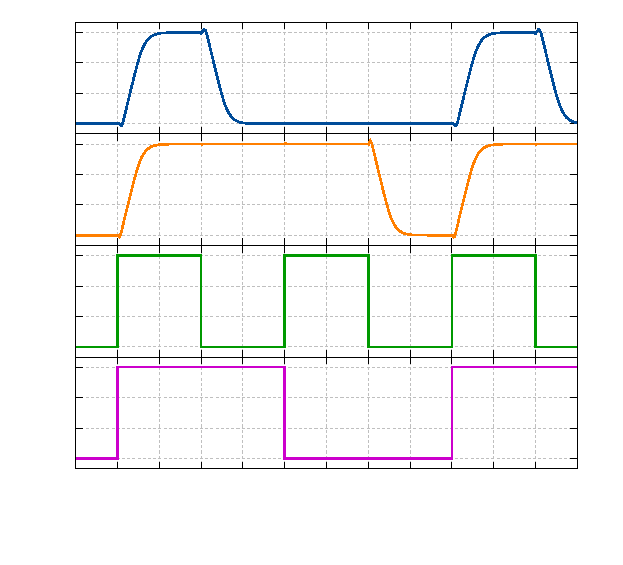
\includegraphics[width={283.40bp},height={198.40bp}]{Immagini/and-or-dinamica}}%
    \gplfronttext
  \end{picture}%
\endgroup

